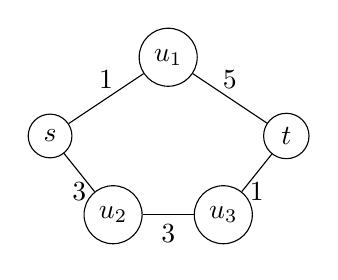
\begin{tikzpicture}
\node[shape=circle,draw=black] (A) at (0,0) {$s$};
\node[shape=circle,draw=black] (U1) at (1.5,1) {$u_1$};
\node[shape=circle,draw=black] (U2) at (0.8,-1) {$u_2$};
\node[shape=circle,draw=black] (U3) at (2.2,-1) {$u_3$};
\node[shape=circle,draw=black] (T) at (3,0) {$t$};

\draw[-] (A)-- node[above] {$1$} ++ (U1);
\draw[-] (A)-- node[below] {$3$} ++  (U2);
\draw[-] (U1)-- node[above] {$5$} ++ (T);
\draw[-] (U2)-- node[below] {$3$} ++ (U3);
\draw[-] (U3)-- node[below] {$1$} ++ (T);

\end{tikzpicture}
